% Introduction Checklist:
% - is clear/simple
% - is organized
% - is precise
% - has natural flowing text
% - has begin/middle/end structure
% - all the details from the thesis are presented.
% - provides overall description of the work's contributions
% - provides similarities of current approach vs others.
% - provides differences of current approach vs others.
% - provides advantages of current approach vs others
% - provides overall description of experiments/validation performed.
% - provides overall description of related work
% - identify interest areas of the work (keywords from the title) (in X)
% - context: includes historical evolution of the research topic (in X)
% - context: mentions real world applications related to the research topic (in X)
% - context: move from the move general context to the specific context (in X)
% - contextualize by presenting a basic review from the state-of-the-art (in X)
% - provide motivation for the work. (in X)
% - present the hypothesis being investigated (in X)
% - Solution's fundamental characteristic is presented (in X)
% - Solution's technique/methodology is presented (in X)
% - Solution's advantages are presented (in X)
% - Context for the work is pinned (in Y)
% - The problem being attacked is identified (in Y)
% - The importance of the problem is presented (in Y)
% - Practical applications from the problem are presented (in Y)
% - Presents previous works (in Y)
% - Presents previous work's limitations (in Y)
% - Contributions for the work are defined (in Y)
% - Main results were emphasized (in Y)
% - Text organization was presented (in Y)
% - Previous works are mentioned as non-solves or partial solves
% - Opportunities to group the previous works were acted upon
% - References were sorted numerically

\chapter{Introduction}
\label{chapter:intro}
Team collaboration is ubiquitous in our society, notably within movie and show
producers, scientists, corporate teams, book editors, and even robots
\citep{fields2011analysis, grund2012network, GunnA15, nemoto2011social,
tseng2004novel, wi2009team}. In this context, a crucial problem is \textit{how
to form teams as to maximize their performance}.  For example, a soccer coach
would benefit from composing a team with higher winning odds; a university or
department dean would prefer to fund research teams with higher potential of
producing breakthrough results; and a manager from a company may require to
rearrange a team in order to ramp up productivity. 

The way people form teams is largely influenced by their professional contacts
and past collaborations, i.e., ways in which agents have access to new
information and opportunities. Most teams do not exist in isolation, but within
a social context amidst other teams. Therefore, knowledge of the collaborative
network from people who work in a given context is key information for the team
formation problem.

A social network of agents that collaboratively work in a context emerges when
combining connected co-workers from many different collaboration instances.
This social network formed by agents engaged in \textit{teamwork} can be
mathematically modeled by a graph: a graph $G$ is an ordered pair $G = (V, E)$,
in which $V$ is a set of vertices or nodes and $E$ is a set of edges or lines
between two elements of $V$. Considering the context of movie teams, such graph
can easily be obtained from a movie dataset with records informing cast and
crew. Here, each record features a production team that actively worked
together, and therefore corresponds to a connected set of nodes.

In fact, research using social network analysis in these types of graphs
reveals interesting relationships between topological features from the network
and team performance \citep{Burt04, grund2012network, LiLY2013,
newman2001structure, PapagelisMZ11, stokols2008, uzzi2005collaboration}. Known
topological metrics correlated to team performance involve the study of
structural holes~\citep{Burt04} and the effect of \textit{structural
coefficients} of the entire network~\citep{uzzi2005collaboration}. However,
both studies do not consider the \textit{aggregate} effect of many individual
topological metrics of agents forming teams, nor the \textit{predictive}
capacity of these features with respect to team performance.

Using social network analysis to access the impact of combined social features
in team performance, rather than analyzing social features in isolation, is a
novel perspective that can yield new evidence on how social elements influence
team performance~\citep{aggregation}. Moreover, multivariate analysis works
best when large datasets are employed. Among all, the film industry has one of
the largest and most detailed datasets available: the IMDb (Internet Movie
Database at~\url{http://www.imdb.com}), making it an ideal candidate for the
case analysis. With such a rich dataset, we can perform multivariate predictive
analysis to identify patterns in topological features related to team success.

Finally, teamwork in the film industry is ubiquitous. Teams are responsible for
projects with large budgets that are expected to generate billions in revenue
and impact spectators worldwide~\citep{Ghiassi2015}. Hence, improvements to
movie success forecasting techniques that result from this novel multivariate
research are potentially relevant both in cultural and economic terms.

\section{Motivation}
A simple experiment may point towards the relevance of further investigating
the effect of topological characteristics in team success.
Figure~\ref{fig:pred_intro} shows results of two sample predictors using the
same test/train set. The baseline predictor uses a single training feature: the
previous success of the movie's team members with respect to the parameter
being predicted. The test predictor uses the same feature and an extra
topological one: the total number of people who have previously collaborated
with the movie's team members. Figure~\ref{fig:pred_intro} shows a significant
gain in $R^2$ measures\footnote{The $R^2$  is a  statistical measure of how
well the regression line approximates the real data points.}.

\begin{figure}[tb]\begin{center}
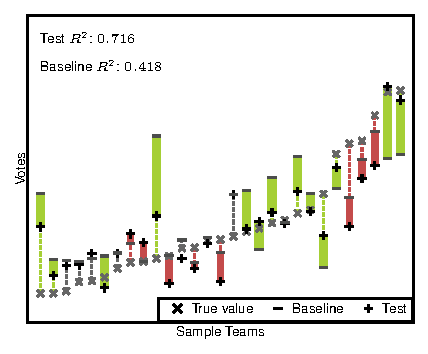
\includegraphics[width=0.6\columnwidth]{../../images/pred_intro2.pdf}
\caption{\label{fig:pred_intro}An example for predictive gain by using a single
extra topological feature. Green and red bars represent prediction error
reduction and increase, respectively.}
\end{center}\end{figure}

Nonetheless, movie success forecasting is not a trivial task because many
complex factors are involved: the quality of special effects, the effectiveness
and range of the movie's marketing campaign, whether it was released on a
holiday, the popularity of its featured actors, and so
on~\citep{elberse2007power,Ghiassi2015}. Additionally, movie success can be
viewed in different ways: the box office (gross generated revenue), its profits
(box office minus budget), its critic and public acclaim, or the movie's
popularity (the number of people who watched the movie). Moreover, success in
one dimension does not guarantee success in the others. This leads to the
proposal of the following hypothesis explored in the present work:

\begin{center}
\emph{In a multivariate predictive analysis of movie success, does using many\\
topological features from teams lead to a more accurate analysis?}
\end{center}

\section{Objectives}
In this thesis, we investigate such hypothesis by analyzing improvements in
movie success prediction models based on multiple social features. To this end,
a social network model is defined from movie production collaborations gathered
from IMDb. Movie success parameters are normalized and social data from teams
is calculated in many different ways. The prediction accuracy of models using
different features from movies and its production teams are also compared.

\section{Contributions}
Our main contribution is a new movie success predictor model for movie
popularity with an $R^2$ score improvement. With this result, we achieve two
main research goals: improving movie success forecasting and high-achieving
team formation. The contributions of this work are summarized as follows.

\begin{itemize}
\item We introduce a network model and selected metrics to assess the
  performance of movie producing teams. We analyze the whole set of movies
  from IMDb and filter it according to well defined features: producer activity,
  release date, type of movie, relevance, team size and connectivity.
\item We define three movie success parameters based on IMDb data (economic
  success, public acceptance and movie popularity) and use them to group all
  movies in three performance categories, which are extensively characterized. 
\item We propose a method for predicting movie success. The prediction task
  considers only features available \textit{before} the movie release.
  Moreover, an important novelty is considering topological features, such as
  structural metrics and constraints related to the production teams' social
  network.
\item Finally, we conduct a thorough evaluation analysis with a complete
  methodology. It is based on evaluating three different regression models
  using fivefold cross validation on balanced train/test sets. We also perform
  feature selection and strength analysis, and identify 23 features that can
  efficiently predict movies success. Our results show that topological
  features\footnote{We use topological and social features interchangeably.}
  extracted from teams provide predictive power.
\end{itemize}

This thesis is organized as follows. Chapter~\ref{chapter:fundamentals}
presents basic information about the dataset employed in this work, along with
key concepts from Social Network analysis, Machine Learning and Statistics.
Chapter~\ref{chapter:related} discusses related work. We present our prediction
model, dataset characterization and strategies for filtering and adjusting its
data in Chapter~\ref{chapter:model}. We then describe our experimental
methodology and analysis in Chapter~\ref{chapter:analysis}. Finally, we present
our discussion, future work and conclusions in
Chapter~\ref{chapter:conclusion}.
